% 
% %\documentclass[paper=a4,fontsize=12pt,open=right,noabbrev]{report}
% \documentclass[12pt]{report}
% \usepackage[utf8]{inputenc}
% \usepackage{amsmath,amsfonts,amsthm}
% \usepackage{amssymb}
% \usepackage{graphicx}
% \usepackage{cite}
% \usepackage{physics}
% \usepackage{mathrsfs}
% \newcommand*\diff{\mathop{}\!\mathrm{d}}
% \usepackage{geometry}
% \usepackage{layouts}
% \usepackage{newfloat}
% \usepackage{float}
% \usepackage{csquotes}
% \setlength{\parindent}{0em}
% \setlength{\parskip}{1em}
% 
% 
% %% Technical point floatstyle
% \floatstyle{ruled}
% \newfloat{Technical Point}{htbp}{lop}[chapter]
% 
% 
% \begin{document}


\chapter{Background}

\section{Statistical Mechanics}
\label{sec:StatMech}
Statistical Mechanics is a branch of physics that deals with complex systems with many degrees of freedom using statistics and probability theory. It emerged from thermodynamics that deals with heat and temperature and is based on three laws that were defined by observing nature.  While this is a macroscopic theory treating temperature and heat as natural quantities, statistical mechanics dives into the microscopic world, resulting in a deeper understanding of the thermodynamic principles. Statistical Physics derives macroscopic matter properties through inference from its microscopic features and marginalising details that are not of importance.~\cite{StatMech}.  

\subsection{Density of States}
\label{sec:DoS}
To understand this view on thermodynamics, we have to define a \textit{microscopic} and \textit{macroscopic} state. We assume a set of $N$  particles in a box, each particle labelled $i$ has a precise position $x_i$ and momentum $p_i$. The microscopic state of a system contains all these information. Mathematically it is a $6N$-dimensional vector in the \textit{phase space} that contains all possible microstates of a system. The phase space grows large even for simple systems of a few particles. Fortunately, the overall information in the system is of minor importance, compared to macroscopic variables, like the system's energy $E$, its volume $V$ and others~\cite{StatMech}. 

Each macroscopic system consists of a large number of possible microscopic states, and it is impossible to determine in which of these states the system is. We define the number of possible states depending on a macroscopic variable as the  \textit{density of states} $\Omega(E,V,..)$. 

\subsection{Ensemble Averages}
\label{sec:EnsembleAv}
We prepare a system and wait for some time such that the system relaxes to \textit{equilibrium}. From a thermodynamical point of view, this means that no heat $Q$ is transferred to or from the system. From a microscopic perspective, we have to assume that the heat can fluctuate but no heat is transferred on average and the distribution of microstates does not change. Only the microstate of the system does change in time.  Hypothetically, one can record all these microstates to find their distribution. Similarly, one may duplicate the equilibrated system with the same macroscopic variables and record the microscopic configuration for each system individually. Both methods give the same answer if the system is \textit{ergodic}. That means that the system can evolve in time and reach any point in phase space with given macroscopic constraints by only passing through allowed states. This can be problematic if, for instance, a constant energy prevents the system from crossing an energy barrier and discovering new states satisfying the constraint. The outcome of the measurement would depend on its initial state. For this reason, we will assume an \textit{ensemble} of the system, i.e. the duplication with equal macroscopic constraints~\cite{StatMech}. 

In practice, it is inconvenient to count microstates in order to find the distribution of microstates. There are three frequently used ensembles in equilibrium statistical mechanics with known probability distribution~\cite{schwabl2006statistische}: 
\begin{itemize}
 \item The microcanonical ensemble of $N$ particles is isolated from the environment and does not exchange energy or particles with it. Each microstate occurs with the probability $p = \frac{1}{N}$.
 \item The canonical ensemble, where the system is connected weakly to a heat bath of constant temperature and interchanges energy with it. The probability distribution is  $p_i = \frac{1}{Z}\exp \left( -\frac{E_i}{k_{\textrm{B}} T} \right ) $, where $Z$ is the normalisation, $k_{\textrm{B}}$ is the Boltzmann constant and $T$ is the temperature of the reservoir and the system.  
 \item The grandcanonical ensemble is connected weakly to a reservoir and interchanges particles and energy with it. The probability distribution is  $p_i = \frac{1}{Y}\exp \left( -\frac{ E_i - \mu N}{k_{\textrm{B}} T} \right )$, where $Y$ is the normalisation and $\mu$ is the chemical potential.
\end{itemize}
The aforementioned probability distributions will not be derived here because they emerge directly from Jaynes Maximum Caliber as presented in the corresponding chapter~\ref{ch:Jaynes}.

Given the probability of all microstates in the system, we could calculate the ensemble average of an observable $O$ by
\begin{equation}
\langle O \rangle = \sum_i^{\text{microstates}} p_i O_i .
\end{equation}
For calculating the probability distribution with respect to the macroscopic observable $O$, we have to sum over all probabilities of all microstates satisfying the observable  
\begin{equation}
 p(O) = \sum_{ i \in O } p_i.
\end{equation}
We note that it is useful to define the density of states according to the controlling parameter of the ensemble, e.g. the energy in the canonical ensemble. In this case we can write
\begin{equation}
 p(O) = \sum_E \frac{\Omega(E,O)}{Z} \exp ( -\frac{E}{k_{\textrm{B}} T}).
\end{equation}
These basic relations open up a way to reweight microstates between ensembles. We assume an energy distribution $p_T(E)$ in canonical ensemble at temperature $T$ sampled from a simulation of a system.  Given above relation, we can reweight the distribution to another temperature $T''$ by
\begin{equation}
\begin{aligned}
 p_{T''}(E) &= \frac{ \Omega(E)}{Z} \exp (-\frac{E}{k_{\textrm{B}} T''}) \\
   &=  \frac{\Omega(E)}{Z'} \exp (-\frac{E}{k_{\textrm{B}} T} + \frac{E}{k_{\textrm{B}} T'} )\\
   &= \frac{p_{T}(E)}{Z'}  \exp (-\frac{E}{k_{\textrm{B}} T'}) ,
\end{aligned}
\end{equation}
using the reference data $p_T(E)$. $T'$ is the shift from the original temperature $T$ to reach the target temperature $T''$. This technique will be derived and discussed using Jaynes Maximum Caliber in chapter~\ref{ch:Jaynes}. 
It relies on knowing the density of states. In fact, the density of states is a starting point to calculate all thermodynamic properties of the system. Therefore, it is the quantity that is of most interest when running a simulation~\cite{janke2013monte}. 


\subsection{Molecular Dynamics}
Simulations are frequently used to discover the phase space of complex systems. Molecular Dynamics (MD) simulations collect information on the micro- and macrostates of the system by numerically solving Newton's equation of motion forward in time.  It is thus of importance to set up the simulation such that the ensemble of choice is sampled correctly. For instance, sampling the canonical ensemble requires to model the heat exchange with the reservoir correctly. Heat is transferred via collision between particles of the system and the reservoir. We do not know when the collision occur so they are modelled using a stochastic variable $\zeta(t)$ acting on the particles in collision. The reservoir and the system are at the same temperature, meaning that each degree of freedom carries  the same amount of energy on average by the equipartition theorem~\cite{schwabl2006statistische}.
\begin{equation}
 m \langle v(t)^2 \rangle = k_{\mathrm{B}} T.
 \label{eq:EquipartitionTh}
\end{equation}
The average energy transferred to the system should be zero, so the stochastic variable has zero mean. Furthermore, weak coupling ensures that collision are uncorrelated and
we write
\begin{equation}
 \begin{aligned}
  \langle \zeta (t) \rangle &= 0 \\
  \langle \zeta_i (t) \zeta_j(t') \rangle &= C \delta (t- t') \delta_{ij} ,
 \end{aligned}
\end{equation}
where $C$ is a constant to be determined and the indices $i,j$ denote single components of a vector. The equation of motion to be solved becomes
\begin{equation}
 m \mathbf{ \ddot x} = -m\gamma \mathbf{ \dot x }+ \boldsymbol{\zeta}(t), 
 \label{eq:Langevin}
\end{equation}
where $m$ is the mass of a particle and $\gamma$ is a constant friction term that dissipates energy. Integrating this equation once gives
\begin{equation}
 \mathbf{\dot x} (t) = \mathbf{v_0} e^{-\gamma t} + \int_0^t e^{\gamma s} \boldsymbol{\zeta(s)} \dd{s},
\end{equation}
where $\mathbf{v_0}$ is the initial velocity. The average over an ensemble is
\begin{equation}
 \langle \mathbf{ \dot x} (t) \rangle = \mathbf{ v_0} e^{-\gamma t}.
\end{equation}
The fluctuation around the average are
\begin{equation}
 \langle (\mathbf{v}(t) - \mathbf{v_0} e^{-\gamma t})^2\rangle = \frac{C}{m^2\gamma} (1-e^{-2\gamma t}).
\end{equation}
Letting the system relax to equilibrium for large $t$ gives the equilibrium fluctuation. Equating these fluctuations with the equipartition theorem in equation~\ref{eq:EquipartitionTh} gives
\begin{equation}
 C = m\gamma k_{\mathrm{B}} T,
\end{equation}
allowing to find the strength of the random force. This ensures fluctuations characteristic for the chosen temperature and sampling the correct ensemble~\cite{pomeau2017langevin}. Note that this derivation uses the fluctuation around the equilibrium value so the thermalisation is not bound to work in off-equilibrium. 

The presented Langevin thermostat is only one possible way of controlling the system, other methods are the DPD thermostat~\cite{soddemann2003dissipative} or the Nos\'{e}-Hoover thermostat~\cite{hoover1985canonical} that can be applied in various equilibrium ensembles. The Langevin equation of the system of interest is numerically integrated using the velocity-verlet algorithm~\cite{verlet1967computer} or the Runge-Kutta method~\cite{kutta1901beitrag} for overdamped dynamics. 


\section{Stochastic Thermodynamics}
\label{sec:StochTherm}
Stochastic thermodynamics is a framework for soft-matter systems under general off-equilibrium conditions: $(i)$ The system is embedded in a liquid solution functioning as a heat-bath with constant temperature $T$, $(ii)$ the system is pushed out of equilibrium with external mechanical forces or unbalanced chemical potentials and $(iii)$ fluctuations play a major role in the system~\cite{seifert2008stochastic}. These assumptions were experimentally verified beyond the linear regime on  particles moved by laser traps~\cite{blickle2006thermodynamics} and DNA or RNA manipulated by optical tweezers~\cite{liphardt2002equilibrium}. 
The main plan is to adapt ideas like heat, entropy, energy and their relations from classical thermodynamics and translate them to the nano- and microscopic world without assuming equilibrium. We start with the Langevin equation for overdamped motion 
\begin{equation}
 \mathbf{\dot x} = \mu \mathbf{ F }( \mathbf{x},\lambda) + \boldsymbol{ \zeta }(t) ,
\label{eq:LangevinOver}
 \end{equation}
where the force $\mathbf{F}(\mathbf{x},\lambda) = \pdv{V(x,\lambda)}{\mathbf{x}} + \mathbf{f}(x,\lambda)$ consists of a conservative and non-conservative part, $\boldsymbol{\zeta}(t)$  is Gaussian noise and $\mu$ is the mobility. The thermal noise is assumed to be independent of the external disturbance  and the temperature of the thermal bath is given by the equilibrium Einstein relation $T = \frac{D}{\mu k_{\mathrm{B}}} $, where $k_{\mathrm{B}}$ is the Boltzmann constant and $D$ is the diffusion coefficient. The parameter $\lambda$ controls an external change of the potential or forces on a system and introduces time-dependent off-equilibrium effects~\cite{seifert2008stochastic}.  



\begin{Technical Point}[t]
  %\setlength{\parindent}{10pt}\noindent 
  The overdamped Langevin Equation~\ref{eq:LangevinOver} can be written in a more general form
  \begin{equation}
   \dd{x} = A(x,t) + B(x,t) \dd{W(t)}, 
  \end{equation}
  where $A(x,t) =\frac{\mu}{m}F(x)$, $B(x,t)= \frac{1}{m}$ and $\dd{W(t)} = \zeta(t) \dd{t}$ being the Wiener process~\cite{van1992stochastic}. The process is reduced to one dimension for simplicity.  The Wiener process is not a continuous function by definition because it integrates over a stochastic variable $W(t)$. Applying Riemann integration to the stochastic term shows
  \begin{equation}
   \lim \limits_{n \to \infty} \sum_j^n B(x,\tau_j) (W(t_{j+1}) -W(t)) ,
  \end{equation}
  where $\tau_j$ lies in $[t_j,t_{j+1}]$. The limit does not exist because W(t) depends on a stochastic variable. The difference in It\^{o} and Stratonovich integration lies in the choice
  \begin{equation}
   \begin{aligned}
    \tau_j &= t_j \;\;\;\;\;\;\;\;\;\;\;\;\;\; &\text{(It\^{o})}&\\
    \tau_j &= \frac{t_j + t_{j+1}}{2}\; & \text{(Stratonovich)}& ,
    \end{aligned}
  \end{equation}
  resulting in different solutions of the integral. The different choices in  $\tau_j$ indicate if the $\delta$-like collision occurs in the beginning or during the discrete time-step. For example, It\^{o} integration is chosen for modelling photon emission or chemical reaction, Stratonovich integration for external effects like connected noise generators~\cite{van1992stochastic}. The latter one is chosen in the present case because the modelled degrees of freedom are much slower than the time between collision. The large amount of collisions imitates the behaviour of noise generators.
  \caption{Stratonovich vs It\^{o} Integration}\label{tec:Strat}
\end{Technical Point}



Initialising the system at some point $\mathbf{x_0}$ and integrating forward in time produces a possible trajectory. We have introduced ensembles for microstates and ensemble averages in the previous section~\ref{sec:EnsembleAv}. We will now do this for the off-equilibrium ensemble defined above. Dynamics of off-equilibrium processes are often time-dependent, so microstates are not sufficient for description and we have to collect trajectories. Through Stratonovich integration (see Technical Point~\ref{tec:Strat}) of equation~\ref{eq:LangevinOver},  we find for the weight of a trajectory $\mathbf{x}(t)$ with starting point $\mathbf{x_0}$\cite{seifert2012stochastic}
\begin{equation}
 p [\mathbf{x}(t),\lambda(t) | \mathbf{x_0}] = \prod_i \exp \left [ - \int_{-t}^t \dd{\tau} \frac{ (\dot x_i - \mu F_i(\mathbf{x},\lambda))^2}{4D} + \frac{\mu}{2} \pdv{F_i(\mathbf{x},\lambda)}{x_i} \right ],
 \label{eq:ptra}
 \end{equation}
where $i$ iterates over all dimension. 
The integration over all trajectories denoted by $\dd{[\mathbf{x}( t)]}$ with initial distribution $p(\mathbf{x_0})$ should be normalised
 \begin{equation}
1= \int \int \dd{\mathbf{x_0}} \dd{[\mathbf{x}( t)]}  p [\mathbf{x}(t),\lambda(t) | \mathbf{x_0}] p(\mathbf{x_0}) .
 \end{equation}
Similarly, one can define the ensemble expectation value over trajectories
\begin{equation}
 \langle O \rangle = \int \int \dd{\mathbf{x_0}} \dd{[\mathbf{x}(t)]} O[\mathbf{x}(t),\lambda(t)]  p [\mathbf{x}(t),\lambda(t) | \mathbf{x_0}] p(\mathbf{x_0}) .
\end{equation}
The action is defined equivalent to equilibrium statistical mechanics by $p[ \mathbf{ x}(t),\lambda(t) ] = \exp (- \mathcal{A}[ \mathbf{ x}(t),\lambda(t) ])$ so one finds from equation~\ref{eq:ptra} 
\begin{equation}
 \mathcal{A} [ \mathbf{x}(t),\lambda(t) ]  = \sum_i \int_{-t}^t \dd{\tau} \frac{ (\dot x_i - \mu F_i(\mathbf{x},\lambda))^2}{4D} + \frac{\mu}{2} \pdv{F_i(\mathbf{x},\lambda)}{x_i} .
\end{equation}
The existence of a trajectory $\mathbf{x}(t)$ implies the existence of the same trajectory under time reversal $\mathbf{\tilde x} (-t)$~\cite{CrooksMicRev}. Time reversal includes a reversed control protocol 
$\lambda (t) \rightarrow \tilde \lambda(-t)$ and trajectories $\mathbf{x}(t) \rightarrow  \mathbf{\tilde x}(-t)$, $\mathbf{\dot x}(t) \rightarrow  \mathbf{ \dot {\tilde {x}}}(-t)$. The action of the reversed trajectory becomes
\begin{equation}
\begin{aligned}
  \mathcal{A} [ \mathbf{  \tilde x}(t), \lambda(t) ] &= \sum_i \int_{-t}^t \dd{\tau} \frac{ \dot x_i^2 + 2\mu F_i(\mathbf{x},\lambda) \dot x_i + F_i(\mathbf{x},\lambda)^2 }{4D} + \frac{\mu}{2} \pdv{F_i(\mathbf{x},\lambda)}{x_i} \\
    &=  \mathcal{A} [ \mathbf{x}(t),\lambda(t) ] + \int_{-t}^t \dd{\tau} \frac{1}{T} \mathbf{F}(\mathbf{x},\lambda) \cdot \mathbf{\dot x}.
\end{aligned}
\end{equation}
The microscopic definition of heat dissipated $q[\mathbf{x}(t),\lambda(t)]$ along a trajectory  can be calculated by the ratio of the weight of a forward trajectory and its time inverted counterpart. The entropy produced in the reservoir $s_m [\mathbf{x}(t),\lambda(t)]$ is related to the heat by dividing with the temperature like in thermodynamics. 
\begin{equation}
\begin{aligned}
 \frac{p [\mathbf{x}(t),\lambda(t) | \mathbf{x}_0]}{p [\mathbf{\tilde x}(t), \tilde \lambda(t) |\mathbf{ \tilde x}_0]} &= \exp \left ( \frac{1}{T} \int_{-t}^t \dd{\tau} \mathbf{F}(\mathbf{x},\lambda) \cdot \mathbf{\dot x} \right ) \\
 &= \exp \left ( \frac{ q [\mathbf{x}(t),\lambda(t)]}{T}  \right ) \\
&= \exp \left ( s_m [\mathbf{x}(t),\lambda(t)]  \right ).
\end{aligned}
\label{eq:microscopicBal}
\end{equation}
The more heat is generated in a forward process, the less likely is the reverse process~\cite{seifert2008stochastic}. This relates forward and time-inverted processes for non-equilibrium processes. Note that this exponential relation implies $s_m [\mathbf{x}(t),\lambda(t)] = -s_m [ \mathbf{\tilde x}(t),\tilde \lambda(t)]$ and therefore, that the heat produced in a forward process is the same as the heat consumed by its time-inverted process and vice versa.   

We expect stochastic thermodynamics to obey the main laws of thermodynamics. The first law states that energy is conserved in an isolated system. A change in internal energy $\Delta U$ consists of heat $Q$ transferred to the system and the work $W$ done by the system on its environment  
\begin{equation}
\Delta U = Q-W .
\end{equation}
for a Langevin process on a microscopic level, this becomes~\cite{sekimoto1998langevin}
\begin{equation}
 \begin{aligned}
  \dd \omega &= \dd u + \dd q\\
             &= \left ( \pdv{V}{\lambda} \dot \lambda \dd{\tau}  \right) + f \dd{x},
  \end{aligned}
  \label{eq:1stlaw}
\end{equation}
where $\dd u$ is identified with $ \pdv{V}{\lambda} \dot \lambda \dd{\tau} $ as the change in potential at fixed particle position and $\dd q$ is identified by $f \dd{x}$ as the heat dissipated by the medium due to the non-conservative force $f$ in agreement to the finding in equation~\ref{eq:microscopicBal}. The second law of thermodynamics states that two initially isolated and equilibrated systems increase their combined entropy when they get in contact. The entropy does not change when the systems were already in equilibrium with each other. 
The second law is validated by defining the total entropy production 
\begin{equation}
\begin{aligned}
 \Delta s_{\text{tot}} [\mathbf{x}(t),\lambda(t),p_{\text{i}},p_{\text{f}}  ] &= \log \frac{p [\mathbf{x}(t) | \mathbf{x}_0] p_{\text{i}}(\mathbf{x}_0)}{p [ \mathbf{\tilde x}(t) | \mathbf{ \tilde x}_0] p_{\text{f}}(\mathbf{ \tilde x}_0)}\\
 &= \log \frac{p [\mathbf{x}(t) | \mathbf{x}_0] }{p [\mathbf{ \tilde x}(t) | \mathbf{ \tilde x}_0] } + \log \frac{p_{\text{i}}( \mathbf{x}_0)}{p_{\text{f}}(\mathbf{\tilde x}_0)}\\
 &= s_m[\mathbf{x}(t),\lambda(t)] + s_{\text{sys}}(p_i,p_f) ,
\end{aligned}
\label{eq:Stot}
\end{equation}
where the distribution change along the trajectory from initial $p_{\text{i}}$ to final $p_{\text{f}}$ is the system contribution to total entropy production. $s_m[\mathbf{x}(t),\lambda(t)]$ is the contribution of the reservoir.  The result is used to derive
\begin{equation}
\begin{aligned}
 \langle \exp \left ( - \Delta s_{\text{tot}} \right ) \rangle &=
 \int \int \dd{\mathbf{x_0}} \dd{[\mathbf{x}( t)]} p_{\text{i}}(\mathbf{x_0}) \exp \left (- \Delta s_{\text{tot}} \right )\\
 &=\int \int \dd{\mathbf{\tilde x_0}} \dd{[\mathbf{ \tilde x}( t)]} p [\mathbf{\tilde x}(t) | \mathbf{\tilde x_0}] p_{\text{f}}( \mathbf{ \tilde x_0})\\
 &= 1 .
\end{aligned}
\label{eq:IFR}
\end{equation}
The second law of thermodynamics $ \langle \Delta s_{\text{tot}} \rangle \geq 0$ follows directly from $\langle \exp - \Delta s_{\text{tot}} \rangle =1 $ . Note that equation~\ref{eq:IFR} does not exclude single trajectories to violate the second law, but these trajectories are exponentially suppressed and the second law is only valid for ensembles of trajectories.   The contributions to entropy production are well separated in contributions of the system and medium, like the first law in equation~\ref{eq:1stlaw}~\cite{seifert2008stochastic}.


\subsection{Transfer Operator}
\label{sec:transferoperator}
The Langevin equation~\ref{eq:Langevin} can produce numerous realisations of a process due to its dependence on a stochastic variable. All of these realisations are possible pathways and are combined in an ensemble of trajectories. A probability distribution $P(x)$ can be constructed depending on the space passing point $x$~\cite{bowman2013introduction}. This distribution is evolved in time according to a generator $\mathscr{L}$,containing all dynamical information by knowledge of a all trajectories passing $x$, denoted by
\begin{equation}
 P(x_{t+\delta t}) = \mathscr{L} \circ  P(x_t).
 \label{eq:operatorcts}
\end{equation} % or so... doesnt nseem right here
The initial probability distribution can be chosen according to physical 
conditions. The infinitesimal generator $\mathscr{L}$ and dependence on the whole history $P(x_t)$ is inconvenient for computational purposes and is approximated by a time-discretised transfer operator.

\subsection{Markov Processes} 
\label{sec:MarkovProp}
We want the transfer operator to evolve the system over a time-range $\tau \gg \delta t$ and we want it to fulfil the \textit{Markov property}. The probability distribution $P(y_i,t_i)$ of a Markov process only depends on the information at the previous time-point $t_{i-1}$. For $n$ successive time-points ($t_1 < t_2 < .. < t_n $) we call
\begin{equation}
 P(t_n, y_n | t_1, y_1 ; t_2, y_2 ; ... ; t_{n-1} , y_{n-1} )=  P(t_n, y_n | t_{n-1} , y_{n-1} )
 \label{eq:transition}
\end{equation}
the time dependent Markovian \textit{transition probability}. Note that the time evolution of a probability distribution can be expressed using the Markov property by the hierarchy
\begin{equation}
 P(t_1, y_1 ; t_2, y_2 ; t_3, y_3 )= P(t_1,y_1) P(t_2, y_2 | t_1 , y_1 ) P(t_3, y_3 | t_2 , y_2 ) ,
 \label{eq:hierarchy}
\end{equation}
where $P(t_1, y_1)$ is the initial probability distribution. The Markov process is fully characterised by knowledge of the transition probabilities and the initial probability distribution.  Integrating over $y_2$ and dividing by $P(t_1,y_1)$ gives
\begin{equation}
 P(t_1, y_1 | t_3, y_3 ) = \int \diff y_2 P(t_2, y_2 | t_1 , y_1 ) P(t_3, y_3 | t_2 , y_2 )
 \label{eq:Chapman}
\end{equation}
where the definition of conditional probabilities was used on the left-hand side \cite{van1992stochastic}. Equation \ref{eq:Chapman} is known as the Chapman-Kolmogorov equation and will be used to test if the Markov property is fulfilled.

The transfer operator with the Markov property is defined by
\begin{equation}
 P_{t+\tau}(y) = \mathscr{T}(\tau) \circ  P_t(x) = \int_\Omega \diff y  W(x|y);\tau)   P_t(y),
\end{equation}
where $\Omega$ represents the full conformational space of the system and $W(x|y;\tau)$ is a transition probability in continuous space from state $y$ to state $x$ after time-step $\tau$.  The operator is related to the time-continuous operator in equation~\ref{eq:operatorcts} by
\begin{equation}
 \mathscr{T}(\tau) = \exp \left ( \mathscr{L} \tau \right ),
\end{equation}
where the eigenvectors $\Psi_i$ of both are the same and the eigenvalue $\lambda_i$ of $\mathscr{T}$ and $\Lambda_i$ of 
$\mathscr{L}$ are related by $\lambda_i = \exp (\tau \Lambda_i)$~\cite{bowman2013introduction}. 

We note that the stationary distribution is reached when  $\mathscr{T}(\tau) \circ  P_s(x) = P_s(x)$, i.e. it is the eigenvector with eigenvalue $1$ of the transfer operator~\cite{schutte2001transfer}. It is assumed to be singular such that the stationary distribution of a system is unique. The smaller eigenvalues are related to the relaxation dynamics of the system, as will be discussed in detail in section~\ref{sec:MSM}.


\subsection{Non-Equilibrium Steady States}
\label{sec:NESS}
A Non-Equilibrium Steady State (NESS) is a special type of non-equilibrium process because the fluxes and population densities do not depend on time. It is generated by driving a system with time-independent non-conservative forces for a long time. The resulting stationary distribution and fluxes are generally unknown. The external driving  results in an input heat flow in the system. The same amount of heat is dissipated in a coupled reservoir to maintain the steady state~\cite{derrida2007non}. The contribution to total entropy production in equation~\ref{eq:Stot} of the system is zero and only the medium produces entropy.

Assuming a Markovian process with transition probability $ W(y|y')$ from state $y'$ to $y$ per unit time,  we may describe the dynamics by the Master equation~\cite{van1992stochastic}
\begin{equation}
\pdv{P(y,t)}{t} = \int \dd{y'} \left ( W(y|y') P(y',t) - W(y'|y) P(y,t) \right ).\end{equation}
The first term on the right hand side of the equation adds up all probability fluxes to state $y$, while the second term adds up all fluxes going out of that state. The result of all probability fluxes is the change in population of that state. We want to deal with NESS, so the time dependence of the distribution is set to $\pdv{P(y,t)}{t} = 0$ . 
Under this condition, the equation can be solved by assuming the fluxes cancel pairwise
\begin{equation}
 W(y|y') P(y',t) = W(y'|y) P(y,t).
\end{equation}
In fact, this is the \textit{detailed balance} condition that holds true in equilibrium systems. However, a general solution can be found by use of the normalisation $\int \dd{y'} W(y'|y) =1$
\begin{equation}
 P(y) = \int \dd{y'}  W(y|y') P(y',t) ,
 \label{eq:GlobalBalance}
\end{equation}
called the \textit{global balance} condition that always holds true for NESS. It shows that the probability to be in a state $y$ is the sum over all probability fluxes from all states. The fluxes transport probability in cycles in the system, unlike for detailed balance where fluxes cancel each other. Note that detailed balance implies global balance but not the other way around~\cite{van1992stochastic}.

We can introduce another NESS condition by integrating the microscopic reversibility condition in equation~\ref{eq:microscopicBal}. The dependence on an external controlling parameter is dropped in a NESS because the disturbance is permanent. For future use, we want to discretise the space. The indicator function assigns each point in space $p$ to a state
  \begin{equation}
    \chi_i (p) =  \begin{cases}
      1\;\;\;\;\; \text{if}\;\;\; p \in i\\
      0\;\;\;\;\; \text{if}\;\;\; p \notin i.
    \end{cases}
  \end{equation}
Each discrete state will be called \textit{microstate}~\cite{bowman2013introduction}, not to be confused with the microstate of statistical physics described in~\ref{sec:StatMech} that consists of all coordinates of every particle in the system. The present microstates emerges from coarse-graining the conformational space. The coarse-grained states can be chosen according to the system studies. In the next step, the probability distribution over entropy production $\Delta S$ for a given transition of microstates is sought. We integrate over all existing trajectories with entropy production $\Delta S $ that start in microstate $i$ and end in microstate $j$. This produces a trajectory ensemble average over all time forward processes, denoted by subscript $F$:
  \begin{equation}
    \begin{aligned}
      P_{ij} ( \Delta S ) 
      =& \int \delta (\chi_i (\mathbf{x}_0)) \dd {\mathbf{x}_0} \int \delta 
(\chi_j (\mathbf{x}_1)) \dd{\mathbf{x}_1} \\ 
      & \int \dd{[\mathbf{x}(t)]}  P (\mathbf{x}_0) p[\mathbf{x}(+t)]  
\delta(\Delta S - \Delta S_F[\mathbf{x}(t)])
    \end{aligned}
  \end{equation}
  where $x_0$ and $x_1$ denotes the start and endpoint of a 
trajectory. Making use of equation~\ref{eq:microscopicBal} transforms the expression to the inverse trajectory ensemble, denoted by subscript $R$:
  \begin{equation}
    \begin{aligned}
      P_{ij} ( \Delta S ) 
      =& \int \delta (\chi_i (\mathbf{x}_0)) \dd{\mathbf{x}_0} \int \delta 
(\chi_j (\mathbf{x}_1)) \dd{\mathbf{x}_1} \\ &  \int \dd{[\mathbf{x}(t)]}   
      P (x_0) p[\mathbf{ \tilde x} (-t)| \tilde \lambda(-t)] e^{\Delta S} 
\delta(\Delta S +  
\Delta S_R ) 
      \\ =& e^{\Delta S} P_{ji}(- \Delta S)  
    \end{aligned}
    \label{eq:DeltaS}
  \end{equation}
where the relation $\Delta S_F = - \Delta S_R$ is used, meaning that the heat gained from the reservoir in a forward trajectory is the same heat ejected for the time-reversed trajectory.  Note, that the probability distributions $P(\mathbf{x}_0)=P(\mathbf{x}_1)$ remain the system  for a non-equilibrium steady state. The resulting equation $\frac{P_{ij}}{P_{ji}}= \exp (\Delta S_{ij})$ relates the amount of heat dissipated or drawn from the reservoir with the probability of the forward and backward jump between predefined microstates, acting like a coarse-grained version of equation~\ref{eq:microscopicBal}. In fact, it is a special case of Crooks fluctuation theorem~\cite{crooks1999entropy} with defined starting and end state in long time approximation. It simplifies to detailed balance in equilibrium when Boltzmann statistics can be assumed.
  
\subsection{Driven Particle in a periodic Potential}
\label{sec:1Dmodel}
The following construction of a \textit{Markov State Model} will be presented on the example of a driven single particle. The model is a simple case of a NESS \cite{speck2007distribution} and consists of a 
particle driven by a non-conservative force $f$ that may emerge from
magnetic fields, mechanical flows, or mechanical dragging. The particle is influenced by a potential shown in figure~\ref{fig:potential1D}.
An analogous experiment was performed using silica spheres on a
tilted crystalline glass substrate \cite{ma2017colloidal}. Another discrete example is a weakly interacting Bose-Einstein condensate on a one-dimensional optical lattice~\cite{labouvie2015non}. The overdamped equation of
motion for the particle is given by
\begin{equation}
0 = -\frac{\partial U( x)}{\partial x} - \gamma \dot x+ \sqrt{2\gamma k_{\mathrm{B}} T} 
\zeta(t) + f,
\end{equation}
where a reservoir of temperature $T$ is coupled to the
system by friction constant $\gamma$ and  $\zeta(t)$ is a $\delta$-correlated
Gaussian process with mean $0$.  Results are presented in reduced units,
where the box size is set to $\mathcal{L}$, the mass of the particle
is set to $\mathcal{M}$, and energy is measured in $\epsilon$. The
temperature is $T = 1\,\epsilon / k_{\mathrm{B}}$, the energy
barriers shown in figure~\ref{fig:potential1D} are varied between $2-4\,\epsilon$ and 
the unit of time is $\mathcal{T} = \mathcal{L}
\sqrt{\mathcal{M}/{\epsilon}}$ .  The integration
time step was set to $\delta t = 10^{-5}\,\mathcal{T}$.  The
non-conservative force is varied between 0 and $9\,\epsilon /
\mathcal{L}$ and the space is separated in 60 microstates of same size.

The presented potential is described by:
\begin{equation}
  \begin{aligned}
  U(x) &=U_0 \left ( \frac{1}{1+\exp(-2k (x-s_{N+1}))} \right ) \\&-  U_N \left ( \frac{1}{1+\exp(-2k (x-s_{0}))} \right ) \\&+ \sum_{j=0}^{j \leq N}  U_j  \left ( \frac{1}{1+ \exp ( -2k (x - s_j  ))}  - \frac{1}{1+ \exp ( -2k (x - s_{j+1}  ))}  \right ) ,
  \end{aligned}
\end{equation}\begin{figure}[t]
\centering
 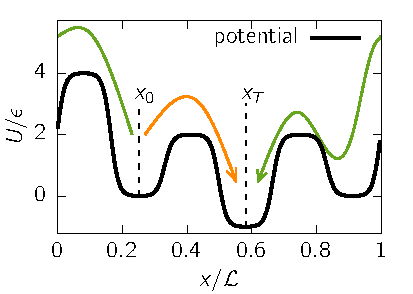
\includegraphics{../plots/Jaynes/potential_traj.pdf}
\caption[An example potential for a driven particle with periodic boundary conditions.]{An example potential, where the minima or chosen to be at position $s_{\textrm{min}}=\frac{3}{12}\,\mathcal{L}, \frac{7}{12}\,\mathcal{L}, \frac{11}{12}\,\mathcal{L}$ with potential minima  $U_{\textrm{min}}= 0\,\epsilon,-1\,\epsilon,0\,\epsilon$ respectively and maxima are at position $s_{\textrm{max}}=\frac{1}{12}\,\mathcal{L}, \frac{5}{12}\,\mathcal{L}, \frac{9}{12}\,\mathcal{L}$ with potential $U_{\textrm{max}}= 4\,\epsilon,2\,\epsilon,2\,\epsilon$ respectively. The green and orange arrow represent two different set of paths going from position $x_i$ to $x_j$. }
\label{fig:potential1D}
\end{figure}where $s_j$ shifts each summand of the potential to its chosen
position, $U_j$ denotes the potential of the $N$ local maxima or minima.
The potential has periodicity $p$ such that $U(x) = U(x+p)$
and $s_{N+1} = s_0 + p$. Parameter $k$ describes the smoothness of the
potential and is chosen as $k = -N \log \left( \frac{1}{0.999} -1
\right)$. $k$ should be chosen larger to minimise a force discontinuity at the periodic boundary. The potential becomes a set of Heaviside steps functions without discontinuity for $k \to \infty$. This potential allows us to construct a model with arbitrary barrier
heights, well depths, steepness of transition regions, and number and position
of wells and barriers. 
  
\subsubsection{Entropy Production}
\label{sec:Sprod}
We want to derive an expression for the local entropy productions $\Delta S_{ij}$ as introduced in \ref{sec:NESS}. The local entropy production of a single continuous trajectory $\mathbf{x}(t)$ is given by 
\begin{equation}
  \label{eq:deltaStraj}
  \Delta S [x (t)] = \int \dd {t} 
  \frac{ \mathbf{F} \cdot \mathbf{ \dot x}}{k_{\mathrm{B}}T},
\end{equation}
where  $\mathbf{ \dot x}$ is the velocity and $T$ is the temperature~\cite{seifert2005entropy}. Making use of numerically discretised trajectories from simulation, $\mathbf{x}(t) \approx \{\mathbf{x}_k\}$, $\Delta S$ is approximated between starting and target points $x_0$ and $x_T$, respectively,
\begin{equation}
 \Delta S[\{x_k \}]\approx \frac{1}{2T} \sum_d \sum_{t=1}^{t=T} \left ( x^{(d)}_t - x^{(d)}_{t-1} \right ) \left ( F^{(d)}({\mathbf{x}}_t) + F^{(d)}({\mathbf{x}}_{t-1}) \right ),
 \label{eq:SprodStr}
\end{equation}
where Stratonovich integration is used (see technical point~\ref{tec:Strat} ) and $d$ iterates over the dimensions.  

The solution above requires to integrate along trajectories and average over a trajectory ensemble. We approximate the  solution by ignoring the fluctuations, allowing us to apply Riemann integration. We make use of the analytic expression ${\mathbf{F}} = - \pdv{U({\mathbf ={x}})}{{\mathbf{x}}} + {\mathbf{f}}$ and find
\begin{equation}
\begin{aligned}
\Delta S [x (t)] &= \frac{1}{k_{\mathrm{B}}T} \int \dd {t} \sum_d \left ( \pdv{U}{x_d} \pdv{x_d}{t} + f_d \pdv{x_d}{t} \right )\\
 &= \frac{1}{k_{\mathrm{B}}T} \int \dd {t} \dv{U}{t} + \sum_d \left ( \int \dd {t} f_d \pdv{x_d}{t} \right )\\
 &=\frac{U(x_T) - U(x_0)  }{k_{\mathrm{B}}T} +  \sum_d \left ( \int \dd {t} f_d \pdv{x_d}{t} \right ) . 
\end{aligned}
\end{equation}
The non-conservative force $\mathbf{f}$ cannot be expressed by a potential and the integral depends on the path of $\mathbf{x}$. For the current 1D-case, two different sets of paths exist between $x_0$ and $x_T$ by using  the periodic boundaries as indicated in figure~\ref{fig:potential1D}. For equilibrium systems with $f=0$ both pathways have the same entropy production, otherwise there are two different solutions. By choosing the time-length of trajectories short, the longer path has negligible weight and we can assume a unique solution to the entropy production. The expression for the local entropy production becomes
\begin{equation}
  \Delta S(x_0,x_T) \approx \frac{ U(x_T) - U(x_0) + (x_T -x_0) f  }{ 
 k_{\mathrm{B}}T },
 \label{eq:Sprodth}
\end{equation}
only depending on start and endpoint of the trajectory. The solution of this equation differs from the solution of equation~$\ref{eq:SprodStr}$ by ignoring fluctuations and giving us an analytic estimate for the entropy production.  The path ensemble average of the entropy production is assumed to agree with the analytic solution as discussed in section~\ref{sec:Trajectory}. The approximated analytic solution is used throughout the thesis as it is much easier to solve. 



  
\section{Markov State Model}
\label{sec:MSM}
Markov State Modeling (MSM) aims to map the slow dynamics of a complex system to an underlying discrete Markovian process.
This involves several steps, including space discretisation, time discretisation and dimensional reduction \cite{bowman2013introduction}. The analysed models in this thesis are constructed such that space discretisation is performed manually.  All steps of the Markov State Model construction are presented on the minimal model introduced in the previous section~\ref{sec:1Dmodel}.

\subsection{Validate Markovian Process}
\label{sec:validate}
Markov processes were introduced in section~\ref{sec:MarkovProp}. An existing process is not bound to fulfill the Markov property so one has to check if it is met using the Chapman-Kolmogorov equation~\ref{eq:Chapman}. We focus on Markov state models of NESS, so the time-dependence on Markovian transition probabilities is dropped. A constant time-step length of each Markovian jump called \textit{lagtime} $\tau$ is assumed. The time-independent Chapman-Kolmogorov equation becomes
\begin{equation}
W(y_i | y_j , n \tau) = \int \diff y_1 \int \diff y_2 ... \int \diff y_{t}  W(y_1 | y_i , \tau) W(y_2 | y_1 , \tau) ...  W(y_j | y_{t} , \tau)
\end{equation}
for $t$ time steps and the transition probabilities depend on the lagtime. The state space of an MSM is discretised so we denote $W(y_i | y_j , \tau) = p_{ij}(\tau)$ as the jump probability from state $i$ to $j$ within time $\tau$. This quantity is estimated from simulation by choosing a lagtime $\tau$ and recording all jumps in a count matrix $c_{ij}(\tau)$. The transition matrix is estimated by
\begin{equation}
 p_{ij}(\tau) = \frac{c_{ij}(\tau)}{\sum_k c_{ik}}.
\end{equation}
In practice, it is cumbersome to check the Chapman-Kolmogorov equation for each element of the matrix $p_{ij}(\tau)$ so Prinz et al. \cite{prinz2011markov} suggested to expand the irreducible transition probability matrix $\hat p(\tau)$ in its eigenvalue decomposition
\begin{equation}
\hat p \boldsymbol{\Phi}_k = \lambda_k \boldsymbol{\Phi}_k .
\end{equation}
The time evolution of the probability distribution can then be described by 
\begin{equation}
 P(t) = \sum_k a_k \boldsymbol{\Phi}_k \exp \left ( -\ln (\lambda_k) t \right ),
 \label{eq:expansion}
\end{equation} 
where $a_k$ are constants that are determined by the initial state of the system. If the dynamics of the system fulfil detailed balance (i.e. the system is in equilibrium), the eigenvalues and eigenvectors are real and one can construct a hierarchy starting with the slowest process $\lambda_0 = 1 > \lambda_1 > ... > 0 $. Typically, the slow dynamical processes are of interested and the fast processes with small $\lambda$ are cut off from the expansion. The characteristic
timescales are identified from equation~\ref{eq:expansion} by $t_i = \frac{-\tau}{\ln \lambda_i}$ and are calculated for different lagtimes. Figure~\ref{fig:lagtime} shows an example of the slowest timescales for varying lagtimes for 60 microstates. The region where $t_i < \tau$ is forbidden because an observed timescale cannot be smaller than the minimal time-resolution of the Markov process.
The timescales reach a plateau for lagtime greater than $ 0.002\,\mathcal{T}$, indicating that the Chapman-Kolmogorov equation~\ref{eq:Chapman} is valid in this region: An MSM at a timescale $\tau_0$ is expected to describe the dynamics for $t > \tau_0$ , so it should agree with
an MSM parameterised at a lagtime $\tau_1 > \tau_0$ describing the same dynamics~\cite{swope2004describing}.  The timescale analysis is merely a tool to choose a lagtime for further analysis.
A test of consistency of the eigenvectors is needed for full conformation of Markovianity.
It is suggested to identify metastable states and compare detailed relaxation probabilities from the MSM to the error-analysed trajectory data. We start by defining the probability distribution of starting in a metastable state $A$ by
\begin{equation}
 \omega^A_i = 
   \begin{cases}
    \frac{\pi_i}{\sum_{j \in A} \pi_j} &\;\;\; i \in A\\
     0 &\;\;\; i \notin A .
   \end{cases}
\end{equation}
The probability of the measured trajectory data to remain in state $A$ after time $m\tau$ is then
\begin{equation}
 L_{\text{tr}}(A,m\tau) = \sum_{i \in A} \omega_i^A \frac{\sum_{j \in A} c_{ij} (m\tau)}{\sum_j c_{ij} (m\tau)},
\end{equation}
with the corresponding error 
\begin{equation}
 \varepsilon(A,m\tau) = \sqrt{m\frac{L_{\text{tr}}(A,m\tau) - \left( L_{\text{tr} }(A,m\tau) \right )^2 }{ \sum_{i \in A} \sum_j c_{ij} (m\tau)} } .
\end{equation}
If the MSM dynamics follows the Markovian relation
\begin{equation}
 \hat p (m \tau) \approx \left [ \hat p(\tau) \right ]^m,
\end{equation}
the result of iterating the MSM 
\begin{equation}
 L_{\text{MSM}}(A,\tau) = \sum_{i \in A} \left [ (\omega_i^A)^\top  [\hat p(\tau)]^m \right ]_i 
\end{equation}
should lie within the errorbars of the trajectory analysis by $L_{\text{tr}}(A,m\tau)$ with error $ \varepsilon(A,m\tau)$  . The method is shown on the 1D model in figure~\ref{fig:Cktest} for full conformation that the model defined by space discretisation and lagtime $\tau$ is Markovian for the slowest processes.
\begin{figure}
\centering
 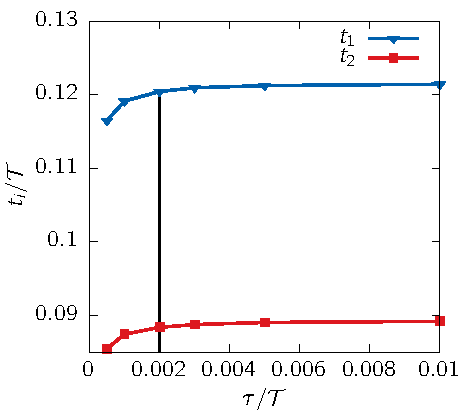
\includegraphics{../plots/MSM/lagtime_2010.pdf}
\caption[Two slowest timescales for the 1D driven system depending on lagtime.]{The slowest two timescales involved in the 1D system, depending on
the lagtime $\tau$ of the MSM. A lagtime of $0.002\,\mathcal{T}$ is chosen for the following analysis. }
\label{fig:lagtime}
\end{figure}

\begin{figure}
\centering
 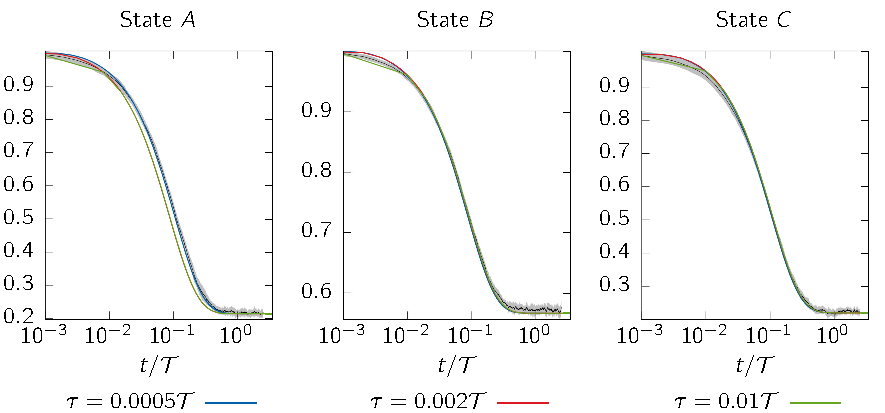
\includegraphics{../plots/MSM/cktest_2010.pdf}
\caption[Chapman-Kolmogorov test for the metastable states for the 1D driven system.]{Chapman-Kolmogorov test for the metastable states $A$,$B$,$C$ . The relaxation processes of the MSM at lagtime $\tau=0.0005\,\mathcal{T},0.002\,\mathcal{T},0.01\,\mathcal{T}$ agree well within the error of trajectory analysis shown by the grey shadow. }
\label{fig:Cktest}
\end{figure}


The eigenvalue decomposition allows detailed analysis of an MSM by isolating each process and showing detailed probability fluxes involved via the corresponding eigenvector.
The described methods rely on the transition probability matrix being reversible, where the eigenvalue decomposition is real-valued. In NESS this condition is not met and the eigenvalues may become
complex. A timescale separation with a hierarchy to delete fast processes with small real part of the eigenvalues is not possible~\cite{weber2017eigenvalues}. A similarly powerful tool
for analysis of NESS is not known yet, however the Schur-decomposition might be a good candidate for timescale separation~\cite{weber2015g}.
In this thesis, a reference equilibrium system is used to choose a lagtime for all driven systems using the same potential surface. First-passage-time-distributions (FPTD) (see section~\ref{sec:FPTD}) characterising the transition time distribution between two metastable states are used for analysis of the processes involved. 

\subsection{Identifying metastable states}
\label{sec:PCCA}
Depending on the number and definition of microstates physical interpretation of MSMs can become difficult. The resulting fine-grained transition matrix does hold all information, but we are only interested in the previously unknown long-term dynamics. The already coarse-grained dynamics can be further coarse-grained to its relevant states. The aim is to combine dynamically well-connected microstates to a macrostate while keeping the timescale of the transitions constant. An often applied method in the field of molecular simulation is the PCCA+~\cite{deuflhard2005robust}, an expansion to the earlier introduced PCCA~\cite{deuflhard1998identification}. We will shortly explain the workflow of PCCA and point out the addition made by PCCA+. 

\begin{figure}[t]
\centering
 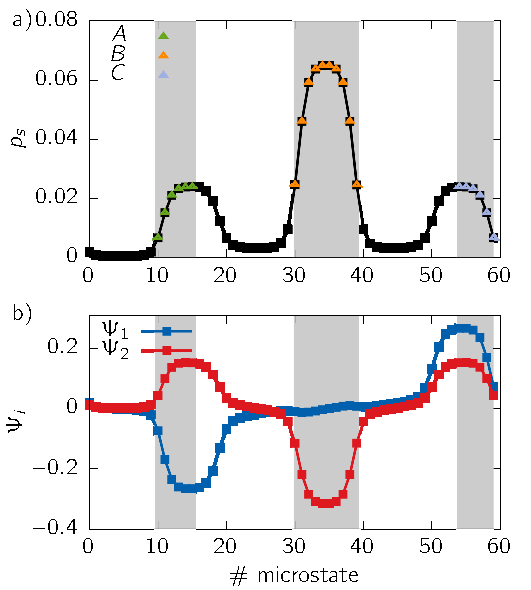
\includegraphics{../plots/MSM/Evec1.pdf}
 \caption{(a) Probability distribution for the equilibrium system with metastable states identified by PCCA+. (b) First and second eigenvector $\Psi_i$ representing the 
 probability flow during relaxation process. }
 \label{fig:Evec}
\end{figure}

By examination of the expansion of $P(t)$ in equation~\ref{eq:expansion}, one understands 
that the processes with $\lambda_i < 1$ vanish with time and only the stationary distribution $\Psi_0$ with $\lambda_0 = 1$ remains. The eigenvalue shows how fast the process annihilates in time, the corresponding eigenvector describes the corresponding probability flow. This is shown in figure~\ref{fig:Evec} for the 1D toymodel. The metastable states are already identified by $A$, $B$ and $C$. The probability flows from states where $\Psi_i$ is positive to the negative region or vice versa, depending on what is needed to reach the steady state. The first eigenvector exchanges probability between metastable state $A$ and $C$, the second between $B$ and $A$, $C$ equally, so the two flows 
cover all transition that one would intuitively expect from the system. 

PCCA makes use of the eigenvector by a hierarchical approach, starting with the eigenvector corresponding to the slowest process. The positive region of $\Psi_1$ is defined as one metastable state and the negative region as another. It continues using the second slowest eigenvector and applies it in the same manner to the metastable state, where it is most active. It proceeds in such a way that the number of metastable states is defined by the number eigenvectors taken into account. This approach is error prone due to large inactive regions where $\Psi_i \approx 0$, that are randomly assigned to one or another metastable state. PCCA+ corrects for this mistake by assuming all eigenvectors at the same time and assigning a membership probability $M$ for each microstate and each metastable state. A microstate between $A$ and $B$ would end up with membership of $M(A) \approx 50\,\%$, $M(B) \approx 50\,\%$ and $M(C) \approx 0\,\%$ due to its positioning as a transition state and should not belong to any metastable state. The states indicated in figure~\ref{fig:Evec}a each have membership $>95\%$ for a state. 

PCCA+ assigns metastable states that may not coincide with the maxima of a probability distribution as demonstrated for state $A$ and $C$. It is focused on making the metastable states dynamically connected, crisp and well separated while keeping the transition timescales between the metastable states constant. To apply the algorithm, the number of metastable states has to be chosen before running PCCA+. Another drawback is that it relies on the property that the 
eigenvalue expansion in equation~\ref{eq:expansion} is real, which only holds for equilibrium system. Similar to the Markovianity check, the metastable states are determined once for the equilibrium system and assumed to be valid for the driven system too. 

\subsection{First-Passage-Time Distribution}
\label{sec:FPTD}

%Include FPTD is more detailed than prinz CK test

First passage-times distributions (FPTD) are widely used to characterise processes in biology, chemistry and physics and are often associated with a free energy barrier a system has to overcome. The FPTD contains detailed transition information by collecting numerous realisations of a process. In experiment and simulation of rare events, the mean of the distribution is given due to limited observed process realisations~\cite{polizzi2016mean}.
Given an MSM with identified metastable states (see section~\ref{sec:PCCA}) the FPTD between all metastable states can be calculated. The collection of initial states is denoted by $I$, of final states by $F$.
For the purpose of calculating the FPTD~\cite{suarez2016estimating} from $I$ to $F$ the MSM is modified such that all final microstates $f \in F$ become a sink, i.e. all jumps out of the metastable state have probability 0 and staying in the state has probability 1
\begin{equation}
\begin{aligned}
\widetilde p_{fj} &= 0 \;\;\; &\forall j\neq f ,\;\;\; \forall f \in F& \\
\widetilde p_{ff} &= 1 \;\;\; &\forall f \in F&.
\end{aligned}
\end{equation}
An initial state is defined, where full probability is in one microstate $i \in I$ of the starting metastable state
\begin{equation}
\begin{aligned}
\rho_{i}^{(0)}  &= 1  \;\;\; & i \in I& \\
\rho_{j}^{(0)}  &= 0 \;\;\; &\forall j \neq i&.
\end{aligned}
\end{equation}
The probability distributions is iterated with the modified Markov model $\widetilde p$ until full probability is trapped in the sink. The superscript of $(t)$ denotes the number of iterations performed.
\begin{equation}
\rho^{(t+1)} = \widetilde p  \rho^{(t)} .
\end{equation}
The first-passage probability $p_{\;\text{FPT}}(t)$ at step $t$ is then the probability flow in the sink 
\begin{equation}
p_{\;\text{FPT}}(i \to F,t) = \sum_{l \in F} \rho^{(t)}_{l} - \rho^{(t-1)}_{l} .
\end{equation}
This calculation is repeated for all initial microstates $i \in I$. The full FPTD is then calculated by weighting each distribution with the weight $w_i$ of a trajectory starting in each initial microstate
\begin{equation}
w_i = \frac{ \sum_{k \notin I } \pi_k p_{ki} }{\sum_{i \in I} \left( \sum_{k \notin I } \pi_k p_{ki} \right ) } ,
\end{equation}
where $\boldsymbol{\pi}$ is the stationary probability distribution of a NESS. 
This expression adds up all probability flow to the initial state $I$ by 
$\sum_{k \notin I } \pi_k p_{ki}$ and normalises the probability of flowing 
into macrostate $I$. Note that this expression does not use the modified 
\begin{figure}[t]
\centering
 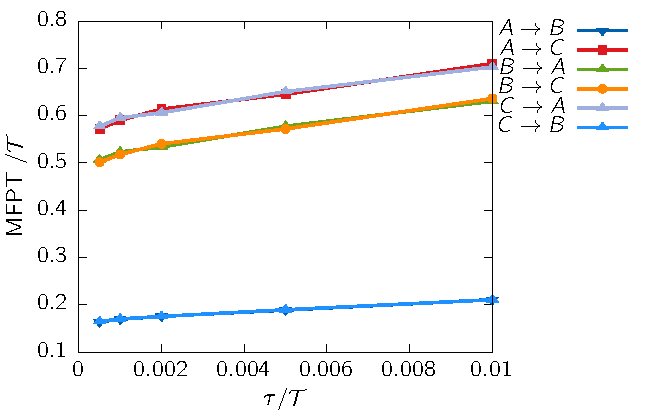
\includegraphics{../plots/MSM/tao_MFPT.pdf}
\caption[Mean first-passage time depending on the lagtime $\tau$ for all six observed processes for the 1D system.]{MFPT depending on the lagtime $\tau$ for all six observed processes. The model is designed such that groups of two processes overlap. The MFPT increases linearly with lagtime for all processes after a short period of faster growth.} 
\label{fig:tau_MFPT}
\end{figure} 
MSM. The full FPT can then be expressed by
\begin{equation}
p_{\;\text{FPT}}(I \to F,t)  = \sum_{i \in I} w_i p_{\;\text{FPT}}(i \to F,t)  .
\end{equation}
Knowing the FPTD, all moments of the distribution can be calculated by
\begin{equation}
M_{I \to F}^{(n)} = \sum_t p_{\text{FPT}} (I \to F,t) t^n.
\end{equation}
In particular we will make use of the quantities
\begin{equation}
 \begin{aligned}
  \mu_{I \to F} &= M_{I \to F}^{(1)} & \;\;\;\text{mean}& \\
  \sigma_{I \to F} &=  \sqrt{M_{I \to F}^{(2)} - \mu_{I \to F}^2 } & \;\;\;\text{standard deviation}& \\
  \kappa_{I \to F} &= \frac{ M_{I \to F}^{(3)} -3 \mu_{I \to F} \sigma_{I \to F}^2-\mu_{I \to F}^3 }{\sigma_{I \to F}^3}& \;\;\;\text{standardised skewness}& ,\\
 \end{aligned}
\end{equation}
where the standardised skewness is defined by the expectation value of $\left( \frac{t-\mu}{\sigma} \right )^3$.
The mean first-passage time (MFPT) was shown to be of special interested because it contains information about the transition rate between two states by the Hill relation~\cite{hill2005free}
\begin{equation}
 k_{I \to F} = \frac{1}{\mu_{I \to F}}.
\end{equation}
Similar to the timescale analysis and the Chapman-Kolmogorov test, the FPTD \begin{figure}[t]
\centering
 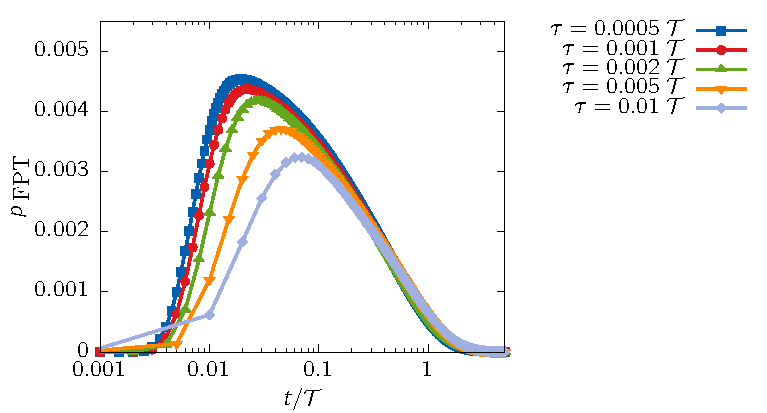
\includegraphics{../plots/MSM/tao_fpt.pdf}
\caption[First-passage time distribution of process from metastable state $B$ to $A$ at different lagtimes.]{FPTD of process from metastable state $B$ to $A$ at different lagtimes. The distributions are normalised such that they can be compared despite different resolution. The distributions do not cover each other, as one would expect from a perfectly Markovian process.}
\label{fig:tau_fpt}
\end{figure}
should not depend on the lagtime in the region of Markovianity. As shown in figure~\ref{fig:tau_MFPT}, this statement does not hold for the given system. The MFPT changes similar to the timescales in figure~\ref{fig:lagtime} up to a lagtime of $\approx 0.002\,\mathcal{T}$ but it continues to grow linearly after this point. The reason for this non-Markovian behaviour is shown in the detailed FPTD in figure~\ref{fig:tau_fpt}.
The increasing lagtime summarises processes that are shorter than $\tau$ but still contribute to the overall MFPT as a single jump and details on the process are lost. The distribution is distorted to slower processes and the MFPT grows. To avoid this problem, the lagtimes should be chosen according to the criterions on Markovianity but as short as possible to keep details on the dynamics. The observed non-Markovianity is detected because the first-passage time is an even stronger test of Markovianity than the test performed in section~\ref{sec:validate}. It analyses transitions between two metastable states and not just the exit from one. The presented exit test is used because it benefits from small error by making use of larger sample sizes. Many trajectories remain in the metastable state for a while. The error increases with time when the amount of trajectories remaining in the basin is small. The error for the FPTD is always large because it requires many incidents of the same transition time and a statistical analysis becomes cumbersome. Irrespective of the discussion of statistical applicability, the non-Markovianity of MFPT raises the question if it is a good quantity for comparison of simulation, MSM and experiment 


 


% 
% 
% 
% % 
% \bibliography{/home/marius/PhD/Thesis/references.bib}
% \bibliographystyle{plain}
% \end{document}
